\documentclass[12pt,a4paper]{article}
\usepackage{cmap} % Makes the PDF copiable. See http://tex.stackexchange.com/a/64198/25761
\usepackage[T1]{fontenc}
\usepackage[brazil]{babel}
\usepackage[utf8]{inputenc}
\usepackage{amsmath}
\usepackage{amsfonts}
\usepackage{amssymb}
\usepackage{amsthm}
\usepackage{textcomp} % \degree
\usepackage{gensymb} % \degree
\usepackage[usenames,svgnames,dvipsnames]{xcolor}
\usepackage{hyperref}
\usepackage{multicol}
\usepackage{graphicx}
\usepackage[margin=2cm]{geometry}
\usepackage{systeme}

\hypersetup{
    colorlinks = true,
    allcolors = {blue}
}

% TODO: Consider using exsheets
% http://linorg.usp.br/CTAN/macros/latex/contrib/exsheets/exsheets_en.pdf
%
% http://ctan.org/tex-archive/macros/latex/contrib/exercise/
% Options: answerdelayed,lastexercise,noanswer
\usepackage[answerdelayed,lastexercise]{exercise}

\addto\captionsbrazil{%
\def\listexercisename{Lista de exerc\'icios}%
\def\ExerciseName{Exerc\'icio}%
\def\AnswerName{Solu\c{c}\~ao do exerc\'icio}%
\def\ExerciseListName{Ex.}%
\def\AnswerListName{Solu\c{c}\~ao}%
\def\ExePartName{Parte}%
\def\ArticleOf{de\ }%
}

\renewcommand{\ExerciseHeaderTitle}{(\ExerciseTitle)\ }
\renewcommand{\ExerciseListHeader}{%\ExerciseHeaderDifficulty%
\textbf{%\ExerciseListName\
\ExerciseHeaderNB.\ %
%\ --- \
\ExerciseHeaderTitle}%
%\ExerciseHeaderOrigin
\ignorespaces}
\renewcommand{\AnswerListHeader}{\textbf{\ExerciseHeaderNB.\ (\AnswerListName)\ }}

\newcommand*\ger[1]{\operatorname{ger}\left\{#1\right\}}
\newcommand*\R{\mathbb{R}}

% Loop Space / CC BY-SA-3.0 / https://tex.stackexchange.com/a/2238/25761
\newenvironment{amatrix}[1]{%
  \left[\begin{array}{@{}*{#1}{c}|c@{}}
}{%
  \end{array}\right]
}

% Loop Space / CC BY-SA-3.0 / https://tex.stackexchange.com/a/3164/25761
%--------grstep
% For denoting a Gauss' reduction step.
% Use as: \grstep{\rho_1+\rho_3} or \grstep[2\rho_5 \\ 3\rho_6]{\rho_1+\rho_3}
\newcommand{\grstep}[2][\relax]{%
   \ensuremath{\mathrel{
       {\mathop{\longrightarrow}\limits^{#2\mathstrut}_{
                                     \begin{subarray}{l} #1 \end{subarray}}}}}}

\renewcommand{\theenumi}{\alph{enumi}}
\renewcommand\labelenumi{(\theenumi) }

\newcommand*\tipo{Prova IV}
\newcommand*\turma{PRO112-02U}
\newcommand*\disciplina{ALI0001}
\newcommand*\eu{Helder G. G. de Lima}
\newcommand*\data{27/06/2018}

\author{\eu}
\title{\tipo - \disciplina}
\date{\data}

\begin{document}
\thispagestyle{empty}
\newgeometry{margin=2cm,bottom=0.5cm}
\begin{center}

\includegraphics[width=9.0cm]{marca} \\
\textbf{\tipo\ (\disciplina / \turma)} \\
Prof. \eu\footnote{
Este é um material de acesso livre distribuído sob os termos da licença \href{https://creativecommons.org/licenses/by-sa/4.0/deed.pt_BR}{Creative Commons BY-SA 4.0}}
\end{center}

\noindent Nome do(a) aluno(a): \underline{\hspace{9,7cm}} Data: \underline{\data}

%\section*{Instruções}
\begin{center}\fbox{
\begin{minipage}{14cm}

{\footnotesize
\begin{itemize}
\renewcommand{\theenumi}{\Roman{enumi}}
\item Identifique-se em todas as folhas.
\item Mantenha o celular e os demais equipamentos eletrônicos desligados durante a prova.
\item Resolva (integralmente) apenas os itens de que precisar para somar 10,0 pontos.
\end{itemize}
}

\end{minipage}
}
\end{center}

\section*{Questões}
\begin{ExerciseList}
\Exercise[title={1,0}]
Explique o que são matrizes semelhantes e dê um exemplo numérico.
\Answer Uma matriz $A$ é semelhante a uma matriz $B$ se existe alguma matriz inversível $P$ tal que $A = P^{-1}BP$. Equivalentemente, $A$ é semelhante a $B$ quando ambas as matrizes representam um mesmo operador linear em relação à bases diferentes.

Por exemplo, se
$B=
\begin{bmatrix}
1 & 2 \\ 3 & 4
\end{bmatrix}$
e
$P=
\begin{bmatrix}
1 & 2 \\ 0 & 1
\end{bmatrix}$
então
$P^{-1}=
\begin{bmatrix}
1 & -2 \\ 0 & 1
\end{bmatrix}$
e a matriz $A$ definida por
$A = P^{-1} B P =
\begin{bmatrix}
7 & -4 \\ 3 & -2
\end{bmatrix}$
é semelhante a $A$.


\Exercise[title={3,0}]
Suponha que um operador linear $T: \R^2 \to \R^2$ transforme os pontos indicados na \autoref{fig:dom} nos pontos correspondentes da \autoref{fig:cd}:
\begin{figure}[h]
    \centering
    \begin{minipage}{0.45\textwidth}
        \centering
        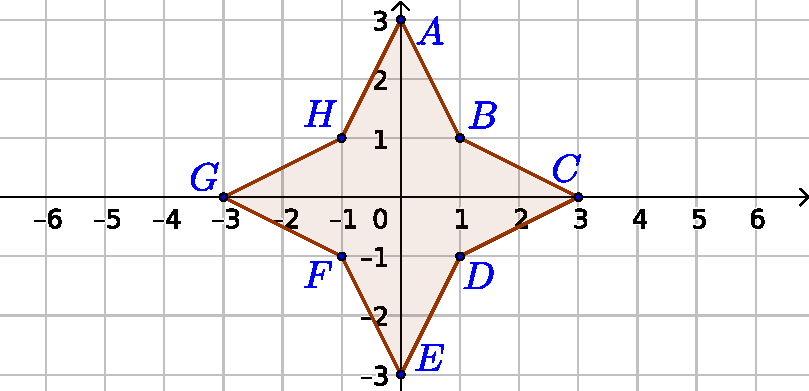
\includegraphics[height=0.48\textwidth]{img/prova-4-pro-plano-dom.pdf}
        \caption{Domínio}\label{fig:dom}
    \end{minipage}\hfill
    \begin{minipage}{0.45\textwidth}
        \centering
        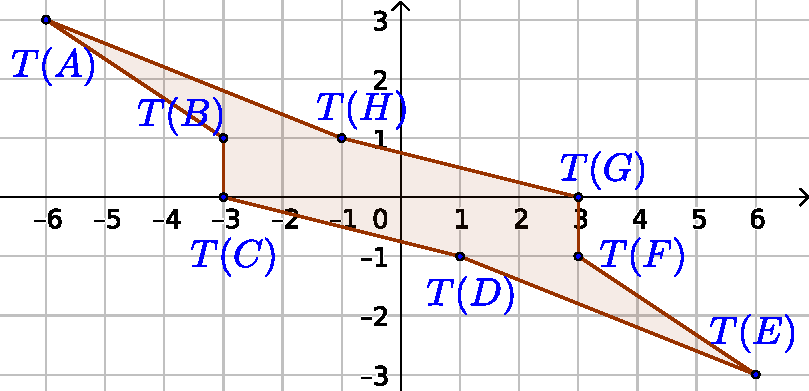
\includegraphics[height=0.48\textwidth]{img/prova-4-pro-plano-img.pdf}
        \caption{Contradomínio}\label{fig:cd}
    \end{minipage}
\end{figure}
\begin{enumerate}
\item Represente os autoespaços de $T$ algebricamente e geometricamente.
\item Existe alguma base $\beta$ de $\R^2$ na qual a matriz de $T$ seja
$\begin{bmatrix}
1 & 0 \\0 & -1
\end{bmatrix}$? Explique.
\end{enumerate}
\Answer
\begin{enumerate}
\item De acordo com as figuras, valem as seguintes relações $T(C) = (-1) \cdot C$ e $T(D) = 1 \cdot D$. Assim, $C$ (e também $G$) é um autovetor de $T$ associado ao autovalor $\lambda_1 = -1$, enquanto que $D$ (e também $H$) é um autovetor associado ao autovalor $\lambda_2 = 1$. Já que o domínio de $T$ tem dimensão 2, estes são todos os autovalores de $T$ e os autovetores $C$ e $D$ geram os autoespaços procurados, isto é,
\begin{align*}
V_{\lambda_1}
& = V_{-1} = \ger{ C } = \{ (3k, 0) \mid k \in \R \} = \text{Eixo horizontal} \\
V_{\lambda_2}
& = V_{1} = \ger{ D } = \{ (k, -k) \mid k \in \R \} = \text{Bissetriz do 2º e 4º quadrantes}
\end{align*}

\item Sim. Já que a matriz dada é uma matriz diagonal, e as entradas da diagonal são os autovalores de $T$, ela é justamente a matriz de T em relação à base $\beta = \{ D, C \} = \{ D, C \} = \{ (3,0), (1,-1) \}$, formada pelos autovetores correspondentes.
\end{enumerate}

\Exercise[title={3,0}]
Seja $T : \R^3 \to \R^3$ o operador linear definido por
\[
T(x,y,z) = (x,x-2y+z,-2y+z).
\]
Verifique se $T$ é diagonalizável, e justifique sua resposta.
\Answer
Como a matriz de $T$ em relação à base canônica é $[T] =
\begin{bmatrix}
1 &  0 &  0\\
1 & -2 &  1\\
0 & -2 &  1
\end{bmatrix}$, o seu polinômio característico é
\begin{align*}
p_{[T]}(\lambda)
= \begin{vmatrix}
\lambda - 1 &          0 &            0\\
        - 1 & \lambda +2 &          - 1\\
          0 &          2 &  \lambda - 1
\end{vmatrix}
& =(\lambda - 1)^2(\lambda +2)+2(\lambda - 1)
  =(\lambda - 1)[(\lambda - 1)(\lambda +2)+2]\\
&=(\lambda - 1)[\lambda^2 +\lambda]
 =(\lambda - 1)(\lambda -(-1))(\lambda-0).
\end{align*}
Assim, os autovalores de $T$ são $1$, $-1$ e $0$. Como $\R^3$ tem dimensão $3$ e $T$ tem três autovalores distintos, resulta que $T$ é diagonalizável.

\Exercise[title={3,0}]
Seja $T: V \to V$ um operador linear. Classifique cada uma das afirmações como \textbf{verdadeira} (e, neste caso, demonstre-a) ou \textbf{falsa} (e dê um contra-exemplo numérico):
\begin{enumerate}
\item Se $v$ é um autovetor de $T$ então $-v$ também é um autovetor de $T$.
\item Se $u$ é um autovetor de $T$ associado ao autovalor $\lambda = 1$ e $w$ é um autovetor de $T$ associado ao autovalor $\lambda = -1$ então $u+w$ é um autovetor de $T$ associado a $\lambda = 0$.
\end{enumerate}
\Answer
\begin{enumerate}
\item \textbf{Verdadeiro}. Se $v$ é um autovetor de $T$ então $T(v) = \lambda v$, para algum $\lambda \in \R$. Logo, $T(-v) = -T(v) = - \lambda v =  \lambda(-v)$ e assim $-v$ também é um autovetor de $T$.
\item \textbf{Falso}. Se $T: \R^2 \to \R^2$ é o operador linear tal que
$
T(1,0) = 1 \cdot (1,0) = (1,0)
$
e
$T(0,1) = (-1) \cdot (0,1) = (0,-1)
$
então $T((1,0) + (0,1)) = T(1,0) + T(0,1) = (1,0) + (0,-1) = (1,-1) \neq (0,0)$.
\end{enumerate}


\Exercise[title={3,0}]
Seja $A = 
\begin{bmatrix}
0 & 0 & 0 \\
1 & 0 & 4 \\
0 & 1 & 0
\end{bmatrix}$. Utilize as propriedades ou teoremas estudados para garantir que $A^3 = 4A$, \textbf{sem calcular a matriz $\mathbf{A^2}$}.
\Answer Como o polinômio característico de $A$ é $ p_A(\lambda) =
\begin{vmatrix}
\lambda & 0 & 0 \\
-1 & \lambda & -4 \\
0 & -1 & \lambda
\end{vmatrix}
=\lambda^3-4\lambda$, segue do Teorema de Cayley-Hamilton que $p_A( A ) = 0$, isto é, que $A^3 - 4A = 0$. Portanto, $A^3 = 4A$.
\end{ExerciseList}

\begin{center}
BOA PROVA E BOAS FÉRIAS!
\end{center}

\newpage
\restoregeometry
\section*{Respostas}
\shipoutAnswer
\end{document}
